\documentclass[11pt]{article}
% motion_header.tex
% include this before the \begin{document} part of your LaTeX source file
%
\usepackage{fourier,ifthen,xspace,amsmath,array}
\usepackage[svgnames, dvipsnames]{xcolor}
\usepackage{graphicx}
\usepackage{siunitx}
\usepackage{xkeyval,calc,moreverb}
\usepackage[breakable,skins]{tcolorbox}
\usepackage{booktabs}
\usepackage{paralist}

% booleans we need
\newboolean{bw}
\setboolean{bw}{false}
\newboolean{solutions}

% counters

\newcounter{problemctr}

% colors

\definecolor{probLineColor}{rgb}{0.2,0.6,0.2}
\definecolor{probLabelColor}{rgb}{0,0,0} % 0.2,0.2,0.7}
\definecolor{probStatementColor}{rgb}{0,0,0}
\definecolor{solColor}{rgb}{0.2,0.6,0.2}

% lengths

\newlength{\probLineWidth} \setlength{\probLineWidth}{1.25pt}
\newlength{\solLineWidth} \setlength{\solLineWidth}{0.5pt}

% oops!
\setlength{\probLineWidth}{0pt}
\setlength{\solLineWidth}{0pt}

% commands

\newcommand{\probdir}{/Users/saeta/Documents/Courses/p24/motion/prob/}
\newcommand{\figdir}{/Users/saeta/Documents/Courses/p24/motion/figs/}
\renewcommand{\probdir}{}
\renewcommand{\figdir}{}
\newcommand{\prob}[2]{% arguments are chapter then problem
  \input{\probdir ch#1/#1P#2}
}

\newcommand{\fig}[2][2]{%
 \vspace*{-.1in}
  \begin{center}%
    \includegraphics[width=#1in]{\figdir#2}
  \end{center}%
}

\newcommand{\SolutionHead}{Solution:}
\newcommand{\theexercise}{}
\newcommand{\PNScolor}[1]{\ifthenelse{\boolean{bw}}{}{\color{#1}}}
\newcommand{\SOL}[1]{\ifthenelse{\equal{#1}{0}}%
  {
\let\solution=\comment
\let\endsolution=\endcomment
\setboolean{solutions}{false}
}%
{\setboolean{solutions}{true}%
\renewenvironment{solution}%
{\par\noindent{\color{solColor}\rule{\linewidth}{\solLineWidth}%
\ifthenelse{\equal{#1}{}}%
{}%
{\par\smallskip\noindent\textbf{\SolutionHead}}}}{}}
}


\newcommand{\val}[2]{\ensuremath{#1~\mathrm{#2}}\xspace}	% number plus unit
\newcommand{\pval}[2]{\ensuremath{\left(#1~\mathrm{#2}}\right)\xspace}
\newcommand{\hval}[2]{\ensuremath{#1$-$\mathrm{#2}}\xspace}
\newcommand{\dg}[1]{\ensuremath{#1^{\circ}}\xspace}
\newcommand{\half}{\ensuremath{\frac{1}{2}}\xspace}
\newcommand{\ux}{\ensuremath{\mathbf{\hat{x}}}\xspace}
\newcommand{\uy}{\ensuremath{\mathbf{\hat{y}}}\xspace}
\newcommand{\uz}{\ensuremath{\mathbf{\hat{z}}}\xspace}
\newcommand{\ur}{\ensuremath{\mathbf{\hat{r}}}\xspace}
\newcommand{\vv}{\ensuremath{v}\xspace}

\newcommand{\xaxis}{$x$ axis\xspace}
\newcommand{\yaxis}{$y$ axis\xspace}
\newcommand{\zaxis}{$z$ axis\xspace}
\newcommand{\xyplane}{$xy$ plane\xspace}
\newcommand{\xzplane}{$xz$ plane\xspace}
\newcommand{\DOT}{\ensuremath{\boldsymbol{\cdot}}}

\newcommand{\bo}{\ensuremath{\boldsymbol{\omega}}\xspace}
\newcommand{\bO}{\ensuremath{\boldsymbol{\Omega}}\xspace}
\newcommand{\VEC}[1]{\ensuremath{\mathbf{#1}}\xspace}
\newcommand{\AU}{\ensuremath{\mathrm{A.U.}}\xspace}
\newcommand{\DB}{\ensuremath{\mathrm{dB}}\xspace}
\newcommand{\degC}[1]{\ensuremath{#1^{\circ}\mathrm{C}}\xspace}


% environments
\newcommand{\problabel}{Problem}
\newenvironment{problem}[1][]%
{
  \begingroup\refstepcounter{problemctr}
  \ifthenelse{\boolean{solutions}}%
    {
      {\vspace*{-10pt}\noindent\PNScolor{probLineColor}%
        \rule[-5pt]{\linewidth}{\probLineWidth}}
    }{}
  \begin{list}{%
      \PNScolor{probLabelColor}\textbf{\problabel\theexercise}%
    }{%
      \setlength{\labelsep}{0pt}%
      \setlength{\leftmargin}{0in}%
      \setlength{\labelwidth}{0pt}%
      \setlength{\listparindent}{0pt}
    }%
    \PNScolor{probStatementColor}%
	\item%
	\ifthenelse{\equal{#1}{}}%
      {}%
      {\textbf{ -- #1}}%
      \quad
}%
{%
  \end{list}\endgroup%
  \PNScolor{black}%
}

\newcommand{\PAGE}[2]{#1-#2\xspace}

\newenvironment{solution}{}{}
\newenvironment{question}{\renewcommand{\problabel}{Question}\begin{problem}}
{\end{problem}\renewcommand{\problabel}{Problem}}

\SOL{1} % show solution

\makeatletter
\newlength\rpLW
\newlength\rpRW
\newlength\rpgap
\newcommand{\rprcent}{0}
\newcommand{\rplcent}{0}
\define@key{rp}{lwidth}{\setlength{\rpLW}{#1}  \setlength{\rpRW}{\columnwidth-#1-\rpgap}}
\define@key{rp}{rwidth}{\setlength{\rpRW}{#1} \setlength{\rpLW}{\columnwidth-#1-\rpgap}}
 \define@key{rp}{lvert}{\def\LeftVerticalCode{#1}}
\define@key{rp}{rvert}{\def\RightVerticalCode{#1}}
\define@key{rp}{gap}{\setlength{\rpgap}{#1}}
\define@key{rp}{rcent}{\def\rprcent{#1}}
\define@key{rp}{lcent}{\def\rplcent{#1}}
\setkeys{rp}{rwidth=2in, lvert=c, rvert=t, gap=0.25in, rcent=0, lcent=0}
\makeatother

\newcommand\rp[3][]{%
  \setkeys{rp}{#1}
  \noindent \parbox[\LeftVerticalCode]{\rpLW}%
  {\ifthenelse{\equal{\rplcent}{0}}%
  {#2}%
  { \begin{center}#2\end{center} }%
  }%
  \hspace*{\rpgap}%
  \parbox[\RightVerticalCode]{\rpRW}%
  {\ifthenelse{\equal{0}{\rprcent}}%
  {#3}%
  {\begin{center} #3 \end{center}}}%
}

\newcommand{\DD}{\ensuremath{d}}		% differential d without leading space
\newcommand{\dd}{\ensuremath{\,\DD}}	% differential d

\newcommand{\deriv}[3][]{\ensuremath{%
	\ifthenelse{\equal{#1}{}}{\frac{\DD #2}{\DD #3}}
	{\frac{\DD^{#1} #2}{\DD #3^{#1}}}}}

\newcommand{\pd}[3][]{\ensuremath{%
	\ifthenelse{\equal{#1}{}}{\frac{\partial #2}{\partial #3}}
	{\partial #2 / \partial #3}}}

\newcommand{\so}{\ensuremath{\qquad\Longrightarrow\qquad}}
\newcommand{\uth}{\ensuremath{\boldsymbol{\hat{\theta}}}\xspace}
\newcommand{\eref}[2][]{%
	\ifthenelse{\equal{#1}{}}%
	{Eq.~(\ref{eq:#2})}%
	{Equation~(\ref{eq:#2})}\xspace}
\newcommand{\cross}{\ensuremath{\times}\xspace}
\newcommand{\into}{\ensuremath{\hat{\otimes}}}	% direction symbols
\newcommand{\outof}{\ensuremath{\hat{\odot}}}
\newcommand{\ds}{\displaystyle}

\newcommand{\xdd}{\ensuremath{\ddot{x}}\xspace}
\newcommand{\thdd}{\ensuremath{\ddot{\theta}}\xspace} % Download this file from physics.hmc.edu/motion/ page
\usepackage{tikz}

\usetikzlibrary{arrows,calc}
                	\tikzset{%
                         every picture/.style={>=stealth'},
                                        vel/.style={->,line width=2pt,color=DarkBlue},
                  force/.style={line width=1.5pt,color=blue,->},
                  coord/.style={color=green!40!black,|->},
                  accel/.style={->,line width=3pt,color=gray},
                  photon/.style={line width=1.5pt,color=DarkRed,decorate,decoration={snake,post length=0.1in}},
                  spring/.style={decorate,decoration={coil,aspect=0.3,segment length=2mm,amplitude=2mm}},
                  traj/.style={dashed, color=gray, line width=1pt}
                }
                
\usepackage{fullpage}
\setlength{\parskip}{6pt}
\setlength{\parindent}{0pt}
\usepackage[margin=1in]{geometry}
\usepackage{graphicx}
\usepackage{enumerate}
\usepackage{marvosym}
\usepackage{amssymb}
\usepackage{wasysym}
\usepackage{gensymb}
\usepackage{mathrsfs}
\usepackage{scrextend}
\usepackage{mathtools}
\usepackage{pgfplots}
\usepackage{xspace}
\usepackage[colorlinks]{hyperref}

% --- style --- %
\renewcommand{\labelenumi}{{ (\alph{enumi})}}
\newcommand{\sand}{\quad \mbox{ and } \quad}
\newcommand{\be}{\begin{enumerate}[a) ]}
\newcommand{\ee}{\end{enumerate}}
\def\bal#1\eal{\begin{align*}#1\end{align*}}
\allowdisplaybreaks

% --- making \xi look less awful --- %
\DeclareSymbolFont{CMletters}{OML}{cmm}{m}{it}
\DeclareMathSymbol{\xi}{\mathord}{CMletters}{"18}

% --- math --- %
\newcommand{\Z}{\mathbb{Z}}
\newcommand{\R}{\mathbb{R}}
\newcommand{\C}{\mathbb{C}}
\newcommand{\Q}{\mathbb{Q}}


\newcommand{\Lt}[1]{\mathcal{L}\crb{#1}}
\newcommand{\ilt}[1]{\mathcal{L}^{-1}\crb{#1}}

\newcommand{\pn}[1]{\left( #1 \right)}
\newcommand{\sqb}[1]{\left[ #1 \right]}
\newcommand{\crb}[1]{\left\{ #1 \right\}}
\newcommand{\lra}[1]{\left\langle #1 \right\rangle}
\newcommand{\magn}[1]{\left\lVert #1 \right\rVert}

\def\multiset#1#2{\ensuremath{\left(\kern-.3em\left(\genfrac{}{}{0pt}{}{#1}{#2}\right)\kern-.3em\right)}}

\newcommand{\pdr}[2]{\frac{\partial #1}{\partial #2}}
\newcommand{\im}[1]{\text{im}\pn{#1}}
\newcommand{\m}[1]{\Z/#1\Z}


\DeclareMathOperator{\proj}{proj}
\newcommand{\vectorproj}[2][]{\proj_{\VEC{#1}}\VEC{#2}}

\newenvironment{amatrix}[1]{%
  \left(\begin{array}{@{}*{#1}{c}|c@{}}
}{%
  \end{array}\right)
}

\makeatletter
\renewcommand*\env@matrix[1][*\c@MaxMatrixCols c]{%
  \hskip -\arraycolsep
  \let\@ifnextchar\new@ifnextchar
  \array{#1}}
\makeatother

\newcommand{\spn}[1]{\text{span}\pn{#1}}

\newcommand*\Heq{\ensuremath{\overset{\kern2pt H}{=}}}

\newcommand{\distil}{\sqrt{1-v^2/c^2}}
\newcommand{\distilf}[1]{\sqrt{1-(#1)^2}}
\newcommand{\lorentz}{\frac{1}{\distil}}
\newcommand{\lorentzf}[1]{\frac{1}{\sqrt{1-(#1)^2}}}

\begin{document}

\noindent{\large Problem Set 4, 1 October 2018\hfill Name: Thomas Martinez ,  Section: 9 }
\vspace*{0.25in}


\begin{problem}[(P28.10)*]
A total amount of positive charge $Q$ is spread onto a nonconducting, flat, circular annulus of inner radius $a$ and outer radius $b$. The charge is distributed so that the charge density (charge per unit area) is given by $\sigma = k/r^3$, where $r$ is the distance from the center of the annulus to any point on it. Show that (with $V=0$ at infinity) the potential at the center of the annulus is given by
\[
	V = \frac{Q}{8\pi\epsilon_0} \pn{\frac{a+b}{ab}}.
\]
\end{problem}


% Your solution starts here %%%%%%%%%%%%%%%%%%%%%%%%%%%%%%%%%%%%%%%%%%%%%%%%%%
\textbf{Solution:}\\
We know that $V = \int dV$. Let us first find $Q$ knowing that $dq = \sigma dr$. So,
\bal
	Q &= \int_a^b dq\\
	&=\int_a^b \frac{k}{r^3}2\pi r\,dr\\
	&= 2\pi\int_a^b \frac{k}{r^2}\,dr\\
	&=2\pi k\pn{\frac{1}{a}-\frac{1}{b}}\\
	&= \frac{2\pi k (b-a)}{ab}
\eal
So, we now find $V$ with
\bal
	V &= \int_a^b \frac{dq}{4\pi\epsilon_0 r} \\
	&= \int_a^b \frac{k}{4\pi\epsilon_0 r^3} 2\pi r \,dr\\
	&=\int_a^b \frac{k}{2\epsilon_0 r^2} \,dr\\
	&= \frac{k}{4}\pn{\frac{1}{a^2}-\frac{1}{b^2}}\\
	&=\frac{k(b-a)(a+b)}{4\epsilon_0a^2b^2}\\
	&=\frac{2\pi k(b-a)(a+b)}{8\pi\epsilon_0a^2b^2}\\
	&=\boxed{\frac{Q}{8\pi\epsilon_0}\pn{\frac{a+b}{ab}}.} \tag{Using $Q= \frac{2\pi k (b-a)}{ab}$.}
\eal

% Your solution ends here %%%%%%%%%%%%%%%%%%%%%%%%%%%%%%%%%%%%%%%%%%%%%%%%%%

\clearpage
\begin{problem}[(P28.13)]
On a thin rod of length $L$ lying along the $x$ axis with one end at the origin ($x=0$), as in the figure below, there is a charge per unit length given by $\lambda = kr$, where $k$ is a constant and $r$ is the distance from the origin.
\be
\item Taking the electrostatic potential at infinity to be zero, find $V$ at the point $P$ on the $y$ axis.
\item Determine the vertical component, $E_y$, of the electric field at $P$ from the result of part (a) and also by direct calculation.
\item Why cannot $E_x$, the horizontal component of the electric field at $P$, be found using the result of part (a)?
\item At what distance from the rod along the $y$ axis is the potential equal to one-half the value at the left end of the rod?
\ee
\begin{center}
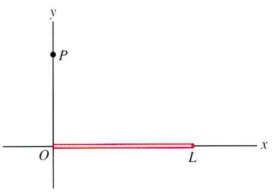
\includegraphics[scale=0.5]{prob2.png}
\end{center}
\end{problem}


% Your solution starts here %%%%%%%%%%%%%%%%%%%%%%%%%%%%%%%%%%%%%%%%%%%%%%%%%%
\textbf{Solution:}\\
\be
\item Let us draw a diagram of how the charge ``goes" to $P$, as well as trying to find an expression for $dq$ and $r_P$.

\vfill

We are given $\lambda = kr$. From our diagram, we see that $\lambda = \frac{dq}{dr}$, so $dq = kr\,dr.$ Also from our diagram, we see that $r_P = \sqrt{r^2+d^2}$. Knowing that $dV = \frac{dq}{4\pi\epsilon_0} r$, we can substitute this with what we know in this problem and get $V$.
\newpage
So,
\bal
V &= \int_0^L \frac{dq}{4\pi\epsilon_0r_P}\\
&= \int_0^L \frac{kr}{4\pi\epsilon_0\sqrt{r^2+d^2}}dr\\
&= \frac{k}{4\pi\epsilon_0} \int_0^L \frac{r}{\sqrt{r^2+d^2}}dr \tag{$u=r^2+d^2$, $du = 2r\,dr$.}\\
&=\frac{k}{4\pi\epsilon_0} \int_0^L \frac{du}{2\sqrt{u}}\\
&=\frac{k}{4\pi\epsilon_0}\pn{\sqrt{r^2+d^2}}\bigg|_0^L\\
V&=\boxed{\frac{k\sqrt{L^2+d^2}}{4\pi\epsilon_0}-\frac{kd}{4\pi\epsilon_0}.}
\eal

\item Let us first find $E_y$ through the result of part (a). We know the relationship $E = -\nabla V$. So, using $d$ as our ``$y$" we can get
\[
	E_y = -\pdr{}{y}V = -\pdr{}{y}\pn{\frac{k\sqrt{L^2+d^2}}{4\pi\epsilon_0}-\frac{kd}{4\pi\epsilon_0}} = \frac{k}{4\pi\epsilon_0} - \frac{kd}{4\pi\epsilon_0\sqrt{L^2+d^2}} \,\VEC{\hat{y}} = \boxed{\frac{k}{4\pi\epsilon_0}\sqb{1-\frac{d}{\sqrt{L^2+d^2}}}\VEC{\hat{y}}.}
\]
Now let us find $E_y$ using direct calculation. We know that $dE = \frac{dq}{4\pi\epsilon_0 r^2}\, \VEC{\hat{r}}$. We have expressions for all these except $\VEC{\hat{r}}$. We know that we only want the $y$ component of $E$, so from the diagram in the previous page, we find that this is equivalent to $\cos\theta$, which is $\cos\theta = \frac{d}{\sqrt{r^2+d^2}}$. So, we find
\bal
	E_y &= \int_0^L \frac{kr}{4\pi\epsilon_0\pn{r^2+d^2}} \frac{d}{\sqrt{r^2+d^2}} \,dr\\
	&= \frac{kd}{4\pi\epsilon_0}\int_0^L\frac{r}{\pn{r^2+d^2}^{3/2}}\,dr \tag{$u = r^2+d^2$, $du = 2r\,dr$.}\\
	&= \frac{kd}{4\pi\epsilon_0}\sqb{-(r^2+d^2)^(1/2)}\bigg|_0^L\\
	&=\frac{kd}{4\pi\epsilon_0}\sqb{\frac{1}{d}-\frac{1}{\sqrt{L^2+d^2}}}\VEC{\hat{y}}\\
	&=\boxed{\frac{k}{4\pi\epsilon_0}\sqb{1-\frac{d}{\sqrt{L^2+d^2}}}\VEC{\hat{y}}.}
\eal
\item Since $P$ is only on the $y$-axis, we are really getting $V$ when we set $x=0$. This means that we cannot find $E_x$ because we cannot find the gradient of a component of $V$, when we only know a single value of that component. It would be like asking to find $f'(7)$ if you are only given $f(7)$, you simply need more information.
\item At the left end of the rod, we note that $d=0$, so we find that the potential $V$ is
\[
	V(0) = \frac{k\sqrt{L^2+d^2}}{4\pi\epsilon_0}-\frac{kd}{4\pi\epsilon_0} = \frac{k\sqrt{L^2+0^2}}{4\pi\epsilon_0}-\frac{k0}{4\pi\epsilon_0} = \frac{kL}{4\pi\epsilon_0}
\]
Now, we need to find at which value $d$ do we get $\frac{1}{2}V(0)$. Let us set this up with
\bal
	V(d) &= \frac{1}{2}V(0)\\
	\frac{k\sqrt{L^2+d^2}}{4\pi\epsilon_0}-\frac{kd}{4\pi\epsilon_0} &= \frac{1}{2}\frac{kL}{4\pi\epsilon_0}\\
	\sqrt{L^2+d^2} - d &= \frac{1}{2}L\\
	\sqrt{L^2+d^2} &= d+\frac{1}{2}L\\
	L^2+d^2 &= d^2+dL+\frac{1}{4}L\\
	L^2 &= dL+\frac{1}{4}L\\
	L^2 - \frac{1}{4}L &= dL\\
	d &= \frac{L^2-\frac{1}{4}L}{L}\\
	 d&= L - \frac{1}{4} = \boxed{\frac{3}{4}L.}
\eal
Let us check this.
\bal
	V(d) &= V\pn{L-\frac{1}{4}}\\
	&= \frac{k\sqrt{L^2+\pn{\frac{3}{4}L}^2}}{4\pi\epsilon_0}-\frac{k\pn{\frac{3}{4}L}}{4\pi\epsilon_0}\\
	&=\frac{k\sqrt{L^2+\frac{9}{16}L^2}}{4\pi\epsilon_0}-\frac{k\pn{\frac{3}{4}L}}{4\pi\epsilon_0}\\
	&= \frac{k\sqrt{\frac{25}{16}L^2}}{4\pi\epsilon_0}-\frac{k\pn{\frac{3}{4}L}}{4\pi\epsilon_0}\\
	&=\frac{k\frac{5}{4}L}{4\pi\epsilon_0}-\frac{k\pn{\frac{3}{4}L}}{4\pi\epsilon_0}\\
	&= \frac{k\frac{1}{2}L}{4\pi\epsilon_0}
\eal
Thus, we know that $V(d) = \frac{1}{2}V(0)$ when $d = \frac{3}{4}L.$
\ee

% Your solution ends here %%%%%%%%%%%%%%%%%%%%%%%%%%%%%%%%%%%%%%%%%%%%%%%%%%

\clearpage

\begin{problem}[\P 3.]
In lecture, we calculated the amount of electrostatic energy contained in the interior
electric field of a uniform sphere of radius $R$ and charge density $\rho$. The result was, 
\[
	U = \frac{2\pi\rho^2}{45\epsilon_0}R^5.
\]
For this problem,  complete the calculation by calculating the energy stored in the \textit{exterior}
electric field, and verify that the \textit{total} stored energy matches the work done to assemble the
sphere.
\end{problem}


% Your solution starts here %%%%%%%%%%%%%%%%%%%%%%%%%%%%%%%%%%%%%%%%%%%%%%%%%%
\textbf{Solution:}\\
From the previous homework, we found that the electric field outside a sphere of constant charge density $\rho$ is
\[
	\VEC{E}_{\text{out}} = \frac{\rho R^3}{3r^2\epsilon_0}.
\]
So, we can find
\[
	u_E = \frac{1}{2}\epsilon_0E^2= \frac{\rho^2 R^6}{18r^4\epsilon_0}
\]
So, we find
\bal
	U_{\text{out}} &= \int_R^{\infty} u_E dV\\
	&= \int_R^{\infty} \frac{\rho^2 R^6}{18r^4\epsilon_0} 4\pi r^2\,dr \tag{$dV = 4\pi r^2\,dr$ from lecture.}\\
	&=\frac{2\pi\rho^2 R^6}{9\epsilon_0} \int_R^{\infty} \frac{1}{r^2}dr\\
	U_{\text{out}} &=\boxed{\frac{2\pi\rho^2 R^5}{9\epsilon_0}.}
\eal
From lecture, we found that the total work done was
\[
	W = \frac{4\pi\rho^2}{15\epsilon_0}R^5.
\]
So, let us verify that the \textit{total} stored energy matches the work done to assemble the
sphere.
\[
	U_{\text{out}} + U_{\text{in}}=\frac{2\pi\rho^2 R^5}{9\epsilon_0}+ \frac{2\pi\rho^2R^5}{45\epsilon_0} = \frac{10\pi\rho^2 R^5}{45\epsilon_0}+ \frac{2\pi\rho^2R^5}{45\epsilon_0} = \frac{12\pi\rho^2 R^5}{45\epsilon_0} = \frac{4\pi\rho^2}{15\epsilon_0}R^5 = W.
\]
Thus, we have verified that the \textit{total} stored energy matches the work done to assemble the
sphere.
% Your solution ends here %%%%%%%%%%%%%%%%%%%%%%%%%%%%%%%%%%%%%%%%%%%%%%%%%%

\clearpage

\begin{problem}[4.]
Consider an infinitely long line of charge with linear charge density $\lambda$ . The line of charge
is parallel to and a distance $d$ above an infinite grounded conducting plane. Sketch the
resulting electric field lines in the half-space above the plane, including any surface
charges. Then using the concepts discussed in lecture, determine the electric field $E(x)$ at
the surface of the plane, as a function of the horizontal distance $x$ from the perpendicular
between the plane and line.
\end{problem}


% Your solution starts here %%%%%%%%%%%%%%%%%%%%%%%%%%%%%%%%%%%%%%%%%%%%%%%%%%
\textbf{Solution:}\\
Let us draw sketch this out.

\vfill

From this, we can imagine that under the grounded conducting plane, there is an identical infinitely long line of charge, but it has linear charge density $-\lambda$. So, we can imagine this sketched out as

\vfill

We know that, for a cylinder of radius $r$ and length $L$, that
\[
	\VEC{E}(r) = \frac{\lambda}{2\pi\epsilon_0r}\VEC{\hat{r}},
\]
where $\lambda=Q/L$. From this, we can calculate $E(x)$ as
\bal
	E(x) &= 2\frac{\lambda}{2\pi\epsilon_0r}\,\VEC{\hat{r}}\\
	&=\frac{\lambda}{\pi\epsilon_0\sqrt{x^2+d^2}}\cos\theta\, \VEC{\hat{-y}}\\
	&=-\frac{\lambda}{\pi\epsilon_0\sqrt{x^2+d^2}}\frac{d}{\sqrt{x^2+d^2}}\, \VEC{\hat{y}}\\
	&=\boxed{-\frac{\lambda d}{\pi\epsilon_0\pn{x^2+d^2}} \,\VEC{\hat{y}}.}
\eal

% Your solution ends here %%%%%%%%%%%%%%%%%%%%%%%%%%%%%%%%%%%%%%%%%%%%%%%%%%

\clearpage

\begin{problem}[5.]
Consider a hollow conducting sphere that carries a net positive charge $Q$. Next, a second
initially uncharged concentric conducting sphere is brought into proximity with the first
(without touching it). In scenario (a), the second sphere is placed outside the first and left
\textit{ungrounded}. In scenario (b), the second sphere is outside the first and \textit{grounded}. In
scenario (c), the second sphere is \textit{inside} the first and also grounded.
\begin{center}
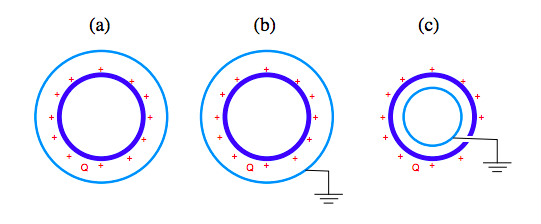
\includegraphics[scale=0.5]{prob5.png}
\end{center}
For all three scenarios, describe the final arrangement of charge on the second sphere and
the electric field (if any) outside the second sphere.
\end{problem}


% Your solution starts here %%%%%%%%%%%%%%%%%%%%%%%%%%%%%%%%%%%%%%%%%%%%%%%%%%
\textbf{Solution:}\be
\item In this configuration, we know that, since the spheres are both conductors there is an induced charge on the inner surface of the ungrounded conducting sphere. However, since it is ungrounded there will also be an induced charge on the outside of the sphere, so there will be an electric field of
\[
	\VEC{E} = \frac{Q}{4\pi\epsilon_0r^2}\,\VEC{\hat{r}}
\]
outside the ungrounded conducting sphere. Here is a sketch:

\item In this configuration, we know that, since the spheres are both conductors there is an induced charge on the inner surface of the grounded conducting sphere. However, since it is grounded, there will NOT be an induced charge on the outside of the sphere, meaning there is no electric field outside the grounded conducting sphere. Here is a sketch:
\vspace{1cm}
\item In this configuration, since the spheres are conductors, there is an induced charge on the outside of the second sphere, and it will be negative. So, outside the second sphere, there will be a negative electric field, but outside the larger sphere, there will be a positive electric field. Here is a sketch:
\ee
% Your solution ends here %%%%%%%%%%%%%%%%%%%%%%%%%%%%%%%%%%%%%%%%%%%%%%%%%%

\clearpage

\begin{problem}[\P 6.]
A cylindrical capacitor is made from two long thin concentric metal cylinders of length $L$
and radii $a$ and $b$. ($L \gg a$ and $a >b$ )
\be
\item Using the definition of capacitance $C =Q/V$ ,	calculate the capacitance per unit
length $C /L$ of this configuration.
\item Repeat the capacitance calculation, this time using the stored energy $U = \frac{1}{2}\frac{Q^2}{C}$.
\ee
\end{problem}


% Your solution starts here %%%%%%%%%%%%%%%%%%%%%%%%%%%%%%%%%%%%%%%%%%%%%%%%%%
\textbf{Solution:}\be
\item We know that, for a cylinder of radius $r$ and length $L$, that
\[
	\VEC{E}(r) = \frac{\lambda}{2\pi\epsilon_0r}\VEC{\hat{r}},
\]
where $\lambda=Q/L$. So, if we want to find capacitance $C$, then we must find the voltage $V$. So, we find $V$ through $V = -\int_a^b E\cdot d\ell$, but $d\ell = dr$ and they are parallel, so we find.
\[
	V = -\int_a^b \frac{Q}{2\pi\epsilon_0rL}dr=\frac{Q}{2\pi\epsilon_0L}\int_b^a\frac{1}{r}dr=\frac{Q}{2\pi\epsilon_0L}\ln\pn{\frac{a}{b}}.
\]
So,
\[
	C = \frac{Q}{V} = \frac{Q}{\frac{Q}{2\pi\epsilon_0L}\ln\pn{\frac{a}{b}}} =\boxed{ \frac{2\pi\epsilon_0L}{\ln\pn{\frac{a}{b}}}.}
\]
\item We know that $U = \int u_E \, dV$ and that $u_E = \frac{1}{2}\epsilon_0 E^2$. We know that $\VEC{E}(r) = \frac{Q}{2\pi\epsilon_0rL}\VEC{\hat{r}}$, so
\[
	u_E = \frac{1}{2}\epsilon_0\frac{Q^2}{4\pi^2\epsilon_0^2r^2L^2} = \frac{Q^2}{8\pi^2\epsilon_0r^2L^2}.
\]
So, 
\bal
	U = \int_b^a u_E \, dV &= \int_b^a \frac{Q^2}{8\pi^2\epsilon_0r^2L^2} 2\pi rL\, dr\\
	&= \int_b^a \frac{Q^2}{4\pi\epsilon_0rL} \, dr\\
	&= \frac{Q^2}{4\pi\epsilon_0L}\int_b^a \frac{1}{r}\,dr\\
	U&= \frac{Q^2}{4\pi\epsilon_0L} \ln\pn{\frac{a}{b}}
\eal
Also, from the relationship from $U = \frac{1}{2}\frac{Q^2}{C}$, we know that $C = \frac{1}{2}\frac{Q^2}{U}$, so
\[
	C = \frac{1}{2}\frac{Q^2}{\frac{Q^2}{4\pi\epsilon_0L} \ln\pn{\frac{a}{b}}} =\boxed{ \frac{2\pi\epsilon_0L}{\ln{\frac{a}{b}}} .}
\]
\ee

% Your solution ends here %%%%%%%%%%%%%%%%%%%%%%%%%%%%%%%%%%%%%%%%%%%%%%%%%%

\clearpage

\end{document}